% -----------------------------------------------------------------
% Document class: Article
\documentclass[ a4paper, twoside, 11pt]{article}
\usepackage{../../../macros-general}
\usepackage{../../../macros-article}
% Number of the handout, quiz, exam, etc.
\newcommand{\numero}{02}
\setcounter{numero}{\numero}

% -----------------------------------------------------------------
\begin{document}
\allowdisplaybreaks

\begin{center}
\Large Mec\'anica Vectorial (MECG-1001): Lecci\'on \numero \\[2ex]
\small \textbf{Semestre:} 2017-2018 T\'ermino II \qquad
\textbf{Instructor:} Luis I. Reyes Castro \qquad
\textbf{Paralelo:} 09
\end{center}
\fullskip

% =============================================
\begin{problem} Dos varillas de 500 mm est\'an conectadas mediante un pasador en $D$ como lo indica la figura de abajo, donde todas las dimensiones se muestran en milimetros. El punto $B$ se mueve hacia la izquierda con una velocidad constante de 360 mm/s. 

\begin{figure}[htb]
\centering
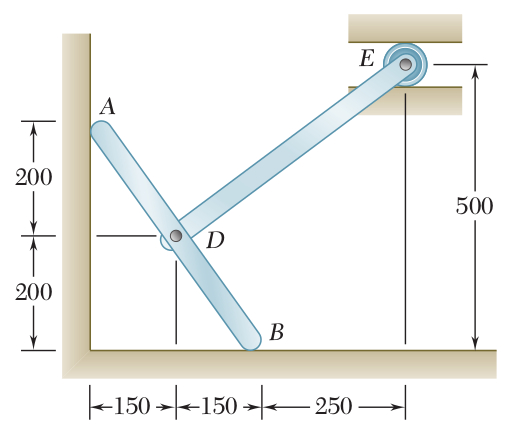
\includegraphics[width=0.46\textwidth]{problema-01.jpg}
\end{figure}

Complete las siguientes actividades: 
\begin{enumerate}[label=\textbf{\alph*)}]
\item \textbf{3 Puntos:} Encuentre la velocidad angular de la barra $AB$. \\[1ex] \emph{Soluci\'on:} Primero tomamos datos: 
\begin{align*}
\vec{v_B} \; & = \; ( \, -0.360, \, 0) \; \text{m/s} \\
\vec{v_A} \; & = \; ( \, 0, \, +v_A) \; \text{m/s} \\
\vec{v_E} \; & = \; ( \, +v_E, \, 0 ) \; \text{m/s} \\
\vec{r_{BA}} \; & = \; ( \, -0.300, \, +0.400 ) \; \text{m} \\
\vec{r_{BD}} \; & = \; ( \, -0.150, \, +0.200 ) \; \text{m} \\
\vec{r_{DE}} \; & = \; ( \, +0.400, \, +0.300 ) \; \text{m}
\end{align*}
Las velocidades en $A$ y $B$ est\'an relacionadas con la velocidad angular de la barra $AB$ de la siguiente manera:
\begin{align*}
& \vec{v_A} \; = \; \vec{v_B} + \vec{\omega_{AB}} \cross \vec{r_{BA}} \\
& \Longrightarrow \; \colvec{0}{+v_A} \; = \; 
\colvec{-0.360}{0} +
\colvec{ -0.400 \, \omega_{AB}}{ -0.300 \, \omega_{AB}} \\
& \Longrightarrow \;
0 \; = \; -0.360 - 0.400 \, \omega_{AB} \\
& \Longrightarrow \;
\vec{\omega_{AB}} \; = \; -0.9 \, \uvec{k} \; \text{rad/s}
\end{align*}
\item \textbf{2 Puntos:} Encuentre la velocidad en $D$. \\[1ex] \emph{Soluci\'on:} Las velocidades en $B$ y $D$ est\'an relacionadas con la velocidad angular de la barra $AB$ de la siguiente manera:
\begin{align*}
\vec{v_D} \; 
& = \; \vec{v_B} + \vec{\omega_{AB}} \cross \vec{r_{BD}} \\
& = \; \colvec{-0.360}{0} +
\colvec{ -0.200 \, (-0.9)}{ -0.150 \, (-0.9)} \\
& = \;
\colvec{ -0.180}{ +0.135} \; \text{m/s} \; \equiv \;
0.225 \; \text{m/s} \; \measuredangle 143.13\deg
\end{align*}
\item \textbf{3 Puntos:} Encuentre la velocidad angular de la barra $DE$. \\[1ex] \emph{Soluci\'on:} Las velocidades en $D$ y $E$ est\'an relacionadas con la velocidad angular de la barra $DE$ de la siguiente manera:
\begin{align*}
& \vec{v_E} \; = \; \vec{v_D} + \vec{\omega_{DE}} \cross \vec{r_{DE}} \\
& \Longrightarrow \; \colvec{+v_E}{0} \; = \; 
\colvec{-0.180}{+0.135} +
\colvec{ -0.300 \, \omega_{DE}}{ +0.400 \, \omega_{DE}} \\
& \Longrightarrow \;
0 \; = \; +0.135 + 0.400 \, \omega_{DE} \\
& \Longrightarrow \;
\vec{\omega_{DE}} \; = \; -0.3375 \, \uvec{k} \; \text{rad/s}
\end{align*}
\item \textbf{2 Puntos:} Encuentre la velocidad en $E$. \\[1ex] \emph{Soluci\'on:} De la expresi\'on anterior tenemos: 
\begin{align*}
\vec{v_E} \;
& = \; \colvec{-0.180}{+0.135} +
\colvec{ -0.300 \, (-0.3375)}{ +0.400 \, (-0.3375)} \\
& = \; \colvec{-0.0788}{0} \; \text{m/s} \; \equiv \;
0.0788 \; \text{m/s} \; \measuredangle \pm180\deg
\end{align*}
\end{enumerate}
\QED

\end{problem}
\fullskip

% =============================================
\begin{problem}
Tres barras, cada una con un peso de 8 lb, est\'an soldadas entre si y se encuentran conectadas mediante pasadores a los dos eslabones $BE$ y $CF$, los cuales tienen peso despreciable y longitud de 10 in. 

\begin{figure}[htb]
\centering
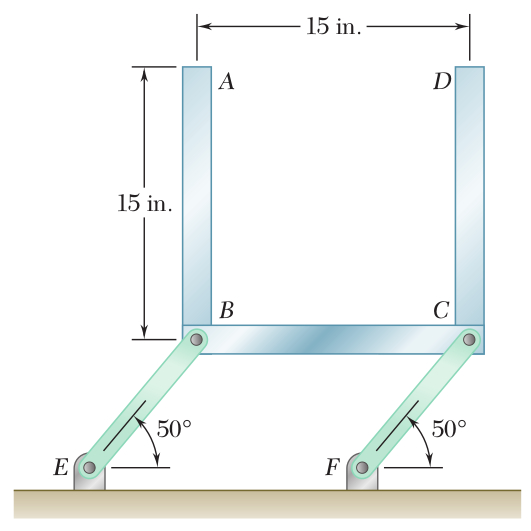
\includegraphics[width=0.46\textwidth]{problema-02.jpg}
\end{figure}

Complete las siguientes actividades: 
\begin{enumerate}[label=\textbf{\alph*)}]
\item \textbf{1 Punto:} Encuentre la locaci\'on del centro de masa del ensamble $ABCD$. \\[1ex] \emph{Soluci\'on:} Es evidente que como el ensamble es sim\'etrico entonces la coordenada $x$ de su centro de masa es igual a la coordenada $x$ del punto medio de la barra $BC$. Para hallar la coordenada $y$ definimos a $\delta$ como la distancia desde el punto medio de la barra $BC$ hasta el centro de masa del ensamble. Entonces tenemos:
\[
\delta \; = \; 
\frac{(8)(0.0) + 2(8)(7.5)}{3(8)} \; = \; 5.0 \; \text{in}
\; = \; 0.4167 \; \text{ft}
\]
\item \textbf{2 Puntos:} Encuentre la aceleraci\'on del centro de masa del ensamble $ABCD$ en funci\'on de la aceleraci\'on angular de la barra $BE$. \\[1ex]
\emph{Soluci\'on:} Primero tomamos algunos datos: 
\begin{align*}
\vec{\hat{r}_{EB}} \;
& = \; ( \, +\cos(50\deg), \, +\sin(50\deg) \, ) \\
\vec{r_{EB}} \;
& = \; 0.8333 \, \vec{\hat{r}_{EB}} \; \text{ft} \\
\vec{\omega_{BE}} \; & = \; \vec{0} \; \text{rad/s} \\
\vec{\alpha_{BE}} \; & = \; \alpha_{BE} \, \uvec{k} \; \text{rad/s\tsup{2}}
\end{align*}
Empezamos reconociendo que el ensamble $ABCD$ se encuentra en translaci\'on curvil\'inea, por lo que en todo momento tanto su velocidad angular como su aceleraci\'on angular son exactamente cero. Consecuentemente: 
\begin{align*}
\vec{a_G} \; = \; \vec{a_B} \; 
& = \; \vec{a_E} + \vec{\alpha_{BE}} \cross \vec{r_{EB}} + \vec{\omega_{BE}} \cross ( \vec{\omega_{BE}} \cross \vec{r_{EB}} ) \\
& = \; \vec{0} + \vec{\alpha_{BE}} \cross \vec{r_{EB}} + \vec{0} \\
& = \; \colvec{ -0.8333 \, \sin(50\deg) \, \alpha_{BE}}{ +0.8333 \, \cos(50\deg) \, \alpha_{BE}}
\end{align*}

\item \textbf{5 Puntos:} Determine la fuerza en cada eslab\'on inmediatamente despu\'es de que el sistema se suelta desde el reposo. \\[1ex]
\emph{Soluci\'on:} Primero tomamos algunos datos: 
\begin{align*}
m \;
& = \; 0.7459 \; \text{slug} \\
\ell / 2 \;
& = \; 7.5/12 \; \text{ft} \; = \; 0.625 \; \text{ft}
\end{align*}
El diagrama de cuerpo libre (DCL) se muestra en la siguiente fotograf\'ia. 
\begin{figure}[htb]
\centering
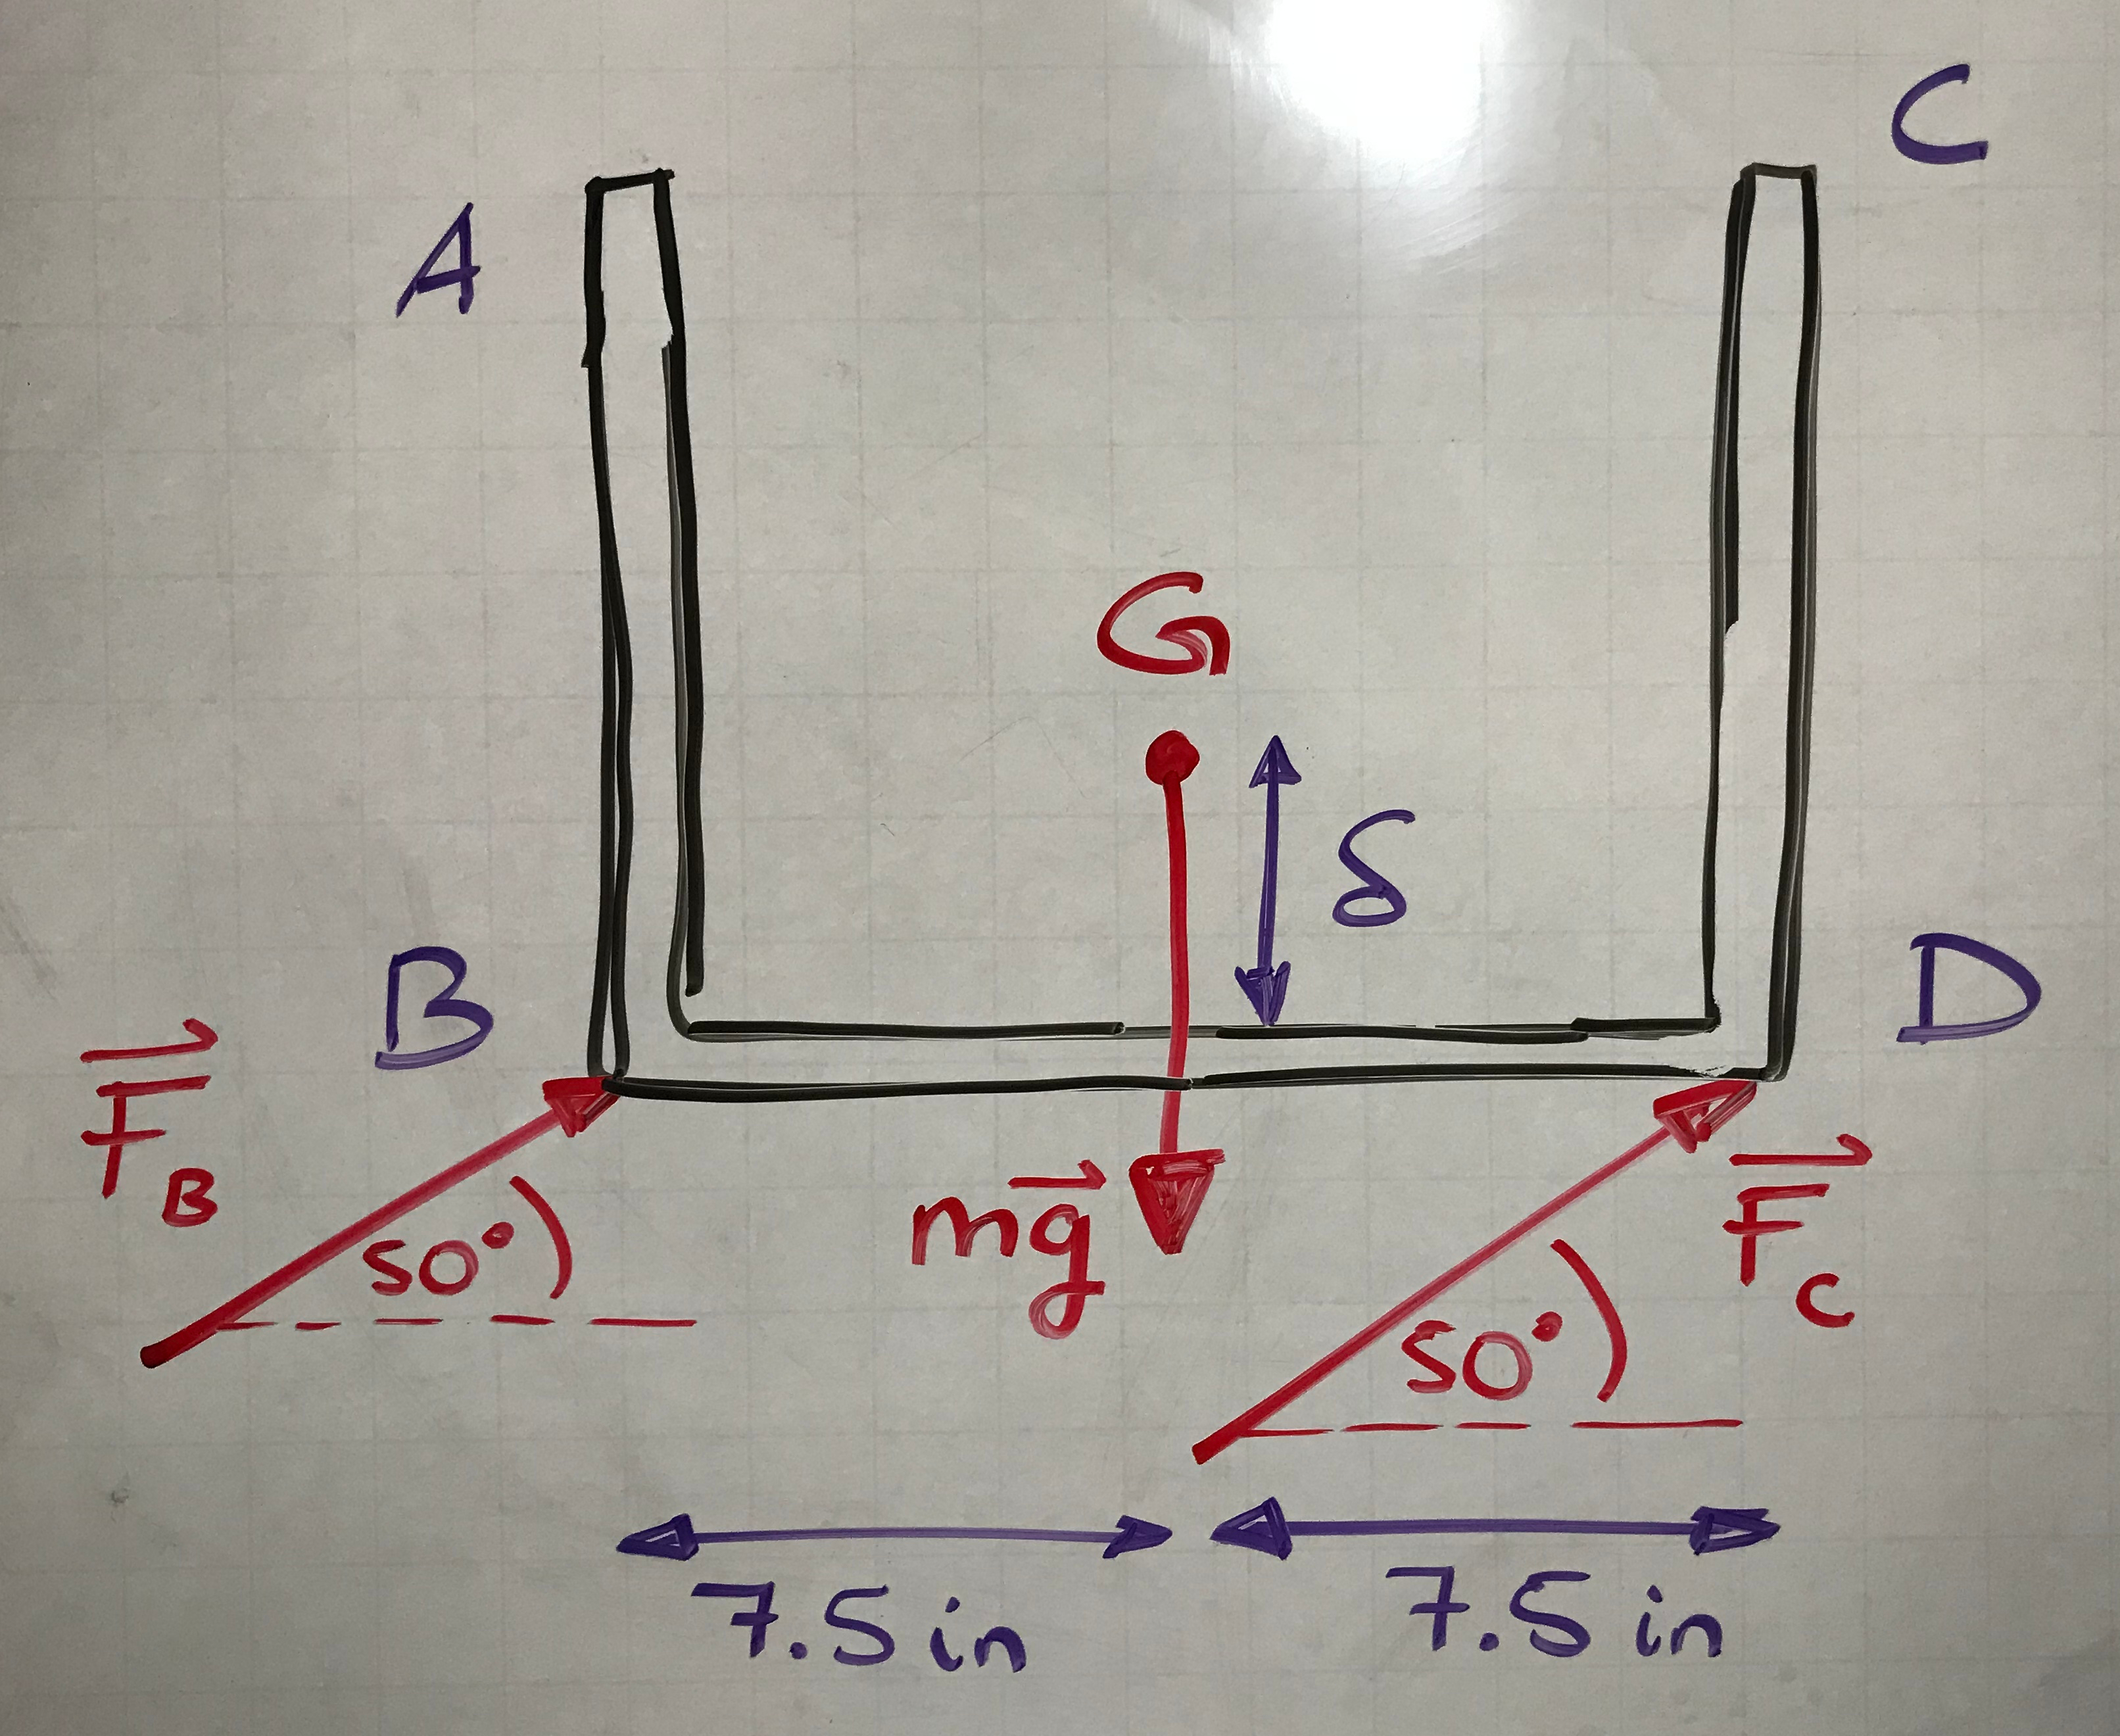
\includegraphics[width=0.44\textwidth]{problema-02_DCL.jpg}
\end{figure}

Las sumatorias de fuerzas y torques externos resultan en: 
\begin{align*}
m \, (\vec{a_G})_x \;
& = \; +(F_B + F_C) \, \cos(50\deg) \\
m \, (\vec{a_G})_y \;
& = \; +(F_B + F_C) \, \sin(50\deg) - mg \\
0 \; & = \; + (\ell/2) \, (F_C - F_B) \, \sin(50\deg) + \delta \, (F_B + F_C) \, \cos(50\deg)
\end{align*}
De esta manera arribamos al siguiente sistema de tres ecuaciones lineales donde las inc\'ognitas son $\alpha_{BE}$, $F_B$ y $F_C$. 
\begin{align*}
-0.6216 \, \sin(50\deg) \, \alpha_{BE} \;
& = \; +(F_B + F_C) \, \cos(50\deg) \\
+0.6216 \, \cos(50\deg) \, \alpha_{BE} \;
& = \; +(F_B + F_C) \, \sin(50\deg) - 24 \\
0 \; & = \; + 0.625 \, (F_C - F_B) \, \sin(50\deg) + 0.4167 \, (F_B + F_C) \, \cos(50\deg)
\end{align*}
Resolviendo el sistema, obtenemos: 
\begin{align*}
\vec{\alpha_{BE}} \;
& = \; -24.82 \; \uvec{k} \; \text{rad/s\tsup{2}} \\
\vec{F_B} & = \; +14.34 \, \vec{\hat{r}_{EB}} \; \text{lb} \\
\vec{F_C} & = \; +4.050 \, \vec{\hat{r}_{EB}} \; \text{lb}
\end{align*}
\end{enumerate}
\QED

\end{problem}
\fullskip

% =============================================
\begin{problem}
\textbf{[6 Puntos]} Los extremos de una barra $AB$ de 9 lb est\'an restringidos a moverse a lo largo de ranuras cortadas en una placa vertical en la forma que se indica. Un resorte de constante $k = 3$ lb/in. se fija al extremo $A$ de manera tal que su tensi\'on es cero cuando $\theta = 0\deg$. La barra se suelta desde el reposo cuando $\theta = 50\deg$, determine la velocidad angular de la barra y la velocidad del extremo $B$ cuando $\theta = 0\deg$. 

\begin{figure}[htb]
\centering
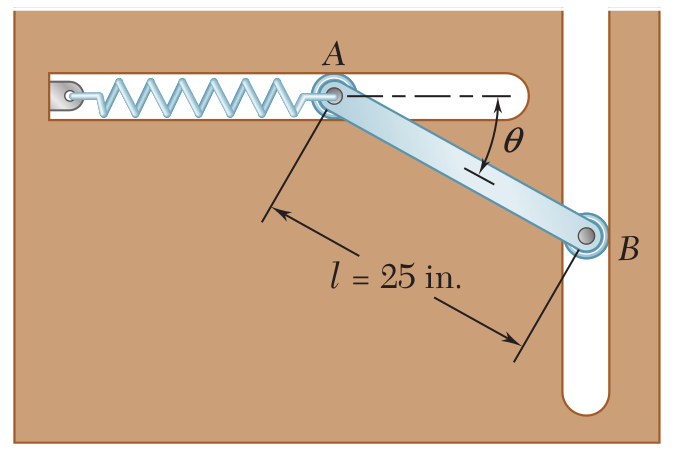
\includegraphics[width=0.5\textwidth]{problema-03.jpg}
\end{figure}

\emph{Soluci\'on:} Primero tomamos algunos datos: 
\begin{align*}
m \; & = \; 0.2797 \; \text{slug} \\
I \; & = \; 0.1012 \; \text{slug-ft\tsup{2}} \\
\ell \; & = \; 2.0833 \; \text{ft} \\
k \; & = \; 36 \; \text{lb/ft}
\end{align*}
Consideraremos que el primer estado del sistema sucede cuando la barra est\'a a $\theta = 50\deg$ y que el segundo estado sucede cuando la barra regresa a $\theta = 0\deg$. Entonces en el segundo estado, tenemos: 
\begin{align*}
\vec{\hat{r}_{AG}} \; & = \; ( \, +1, \, 0 ) \\
\vec{r_{AG}} \; & = \; (\ell/2) \; \vec{\hat{r}_{AG}} \; = \;
1.0417 \; \vec{\hat{r}_{AG}} \\
\vec{r_{AB}} \; & = \; \ell \; \vec{\hat{r}_{AG}} \; = \;
2.0833 \; \vec{\hat{r}_{AG}} \\
\vec{v_A} \; & = \; ( \, -v_A, \, 0 \, ) \; \text{ft/s} \\
\vec{v_B} \; & = \; ( \, 0, \, +v_B \, ) \; \text{ft/s}
\end{align*}
Ahora, la deflecci\'on del resorte y el cambio de altura como funci\'on de $\theta$ puede ser calculados de la siguiente manera: 
\begin{align*}
\Delta x(\theta) \;
& = \; \ell - \ell \, \cos(\theta) \; = \; 
2.0833 \, ( 1 - \cos(\theta) ) \; \text{ft} \\
\Delta h_G(\theta) \;
& = \; (\ell/2) \, \sin(\theta)
\; = \; 1.0417 \, \sin(\theta) \; \text{ft}
\end{align*}
Tambi\'en podemos observar que las velocidades de $A$ y $B$ se relacionan por medio de la velocidad angular de la barra. Esto implica que: 
\begin{align*}
& \vec{v_B} \; = \;
\vec{v_A} + \vec{\omega} \cross \vec{r_{AB}} \\
& \Longrightarrow \;
\colvec{0}{+v_B} \; = \; 
\colvec{-v_A}{0} + \colvec{0}{ +\ell \, \omega} \\
& \Longrightarrow \;
\vec{v_A} \; = \; \vec{0} \; \text{ft/s}
\end{align*}
Consecuentemente: 
\[
\vec{v_G} \; = \;
\vec{v_A} + \vec{\omega} \cross \vec{r_{AG}} \; = \;
\vec{0} + \colvec{0}{ +(\ell/2) \, \omega} \; = \;
\colvec{0}{ +1.0417 \, \omega} \; \text{ft/s}
\]
Es as\'i que la energ\'ia cin\'etica del cuerpo en el segundo estado es: 
\begin{align*}
K_2 \; & = \; 
(1/2) \, m \, v_G^2 + (1/2) \, I \, \omega^2 \\
& = \; (1/2) \, [ \, (0.2797)(1.0417^2) + 0.1012 \, ] \, \omega^2
\; = \; 0.2023 \, \omega^2
\end{align*}
Con todo esto en mente podemos finalmente aplicar el Principio de Trabajo-Energ\'ia. Puesto que ninguna fuerza externa no-conservativa act\'ua sobre el sistema, la energ\'ia del sistema no puede cambiar entre estados. En el primer estado la energ\'ia total est\'a concentrada en la deflecci\'on del resorte: 
\[
E_1 \; = \; (1/2) \, k \, \Delta x(\theta = 50\deg)^2 \; = \;
13.40 \; \text{lb-ft}
\]
En el segundo estado no hay energ\'ia del resorte, sino solamente energ\'ia potencial gravitacional y energ\'ia cin\'etica: 
\[
E_2 \; = \; mg \, \Delta h_G(\theta = 50\deg) + K_2 \; = \;
7.182 + 0.2023 \, \omega^2
\]
Igualando las energ\'ias en los dos estados, y fij\'andonos que en el segundo estado la velocidad angular de la barra es contraria al sentido de las manecillas del reloj, tenemos: 
\[
\vec{\omega} \; = \; +5.544 \; \uvec{k} \; \text{rad/s}
\qquad \Longrightarrow \qquad
\vec{v_B} \; = \; +11.55 \; \uvec{j} \; \text{ft/s}
\]
\QED

\end{problem}
\fullskip

\end{document}